\documentclass[twocolumn]{article}
\usepackage[T1]{fontenc}
\usepackage[utf8]{inputenc}
\usepackage{tabularx,ragged2e,booktabs,caption}
\usepackage{multirow}
\usepackage{color}
\usepackage[top=1in,bottom=1in,left=1.2in,right=1.2in]{geometry}
\usepackage{hyperref}
\usepackage[small]{titlesec}
\usepackage{cite}
\usepackage{graphicx}
\usepackage[autostyle]{csquotes}

\renewcommand\tabularxcolumn[1]{C{#1}}

\newcommand{\todo}[1]{\textcolor{cyan}{\textbf{TODO:} #1}}

\title{CS378: Final Project - Data Artifacts \\ \url{https://github.com/sarimaleem/cs378_fp}}
\author{Sarim Aleem \\ ska2222}

\date{April 27, 2023}

\begin{document}
\maketitle


\begin{abstract}

This paper describes the training and testing of an ELECTRA model for natural
language inference using the Stanford Natural Language Inference Dataset. The
model's performance is benchmarked using contrast sets, and data cartography is
used to improve the model's accuracy. The results show that the base ELECTRA
model performs well on the dataset, and extracting \enquote{ambiguous} examples
from data cartography and training the model on them is an effective method for
improving its performance for some aspects.  We also found that
\enquote{difficult to learn} training examples vastly reduce model performance,
and suggest removing not having them in the training data.

\end{abstract}

\section{Introduction (5pt)}

Natural language inference is the task of determining the truth value of a
hypothesis given a premise. A hypothesis can either be true if it entails from
the premise, false if it contradicts the premise, or neutral if a determination
cannot be made either way. In this paper, train a model based on the Stanford
Natural Language Inference Dataset (SNLI).

We find that the SNLI model has difficulty differenting between neutral labels,
and labels of other classes. We also find that the model often is unable to
contextualize and relate the semantics of different words that have the same
meaning. We created a contrast set in order to test the model, and found that
the performance of the model is significantly degraded in comparison to the
validation set.

In order to reduce ambiguity between words, we decided to train the model on
ambiguous data - data with high variability and medium confidence. We found that
training that although training the model on ambiguous data reduced the models
overall performance by about 3\%, the performance of the model increased on
adversarial data, which in this case are contrast sets, by 3\% as well. We also
found that \enquote{difficult to learn} examples significantly lowered accuracy,
and belive model performance can be improved with them removed.

\section{Task/Dataset/Model Description (15pt)}

The model that was used was the ELECTRA model \cite{clark2020electra}, a
transformer based on BERT. We are training  on the stanford NLI dataset
\cite{bowman2015large}. The dataset has 570000 training examples and 10000
validation examples. The baseline ELECTRA model was fine tuned to the SNLI
training set and was trained with three epochs. We used the default loss
function from the hugging face transformers library. 

For the fix, we took 1655 ambiguous data examples from the first 50000 training
examples and trained on those for 15 epochs on top of the original model. We
also trained 6915 difficult to learn examples for 5 epochs on top of the
baseline model and evaluate that. Our evaluation was accuracy for each of our
different test/validation sets as well as a confusion matrix that describes the
distribution of the data.


\section{Performance Analysis (25pt)}

The model was trained for 3 iterations on the SNLI training dataset. Each
iteration has 550152 training examples, the batch size for the training examples
was 32. All training was done on google colab in the cloud, and training took
about 25 minutes.

\subsection*{Overall Accuracy Statistics}

An initial evaluation of the model shows that it has an accuracy of 88\%. We
also did further evaluation to show statistics about which labels it
misclassified most using a confusion matrix.

\begin{table}[]
\caption{Development Set Evaluation Metrics}
\centering
\begin{tabular}{|l|l|}
\hline
loss       & 0.315   \\ \hline
accuracy   & 0.8865  \\ \hline
runtime    & 20.2629 \\ \hline
examples/s & 485.715 \\ \hline
steps/s    & 60.751  \\ \hline
\end{tabular}
\caption*{\textit{Model Metrics for 9842 examples}}

\caption{Confusion Matrix}
\begin{tabular}{|c|cccc|c|}
\hline
\multicolumn{1}{|l|}{}         & \multicolumn{4}{c|}{\textbf{Predicted}}                                                                              & \multicolumn{1}{l|}{} \\ \hline
\multirow{4}{*}{\textbf{True}} & \multicolumn{1}{l|}{}               & \multicolumn{1}{c|}{\textit{0}} & \multicolumn{1}{c|}{\textit{1}} & \textit{2} & \textbf{Total}        \\ \cline{2-6} 
                               & \multicolumn{1}{c|}{\textit{0}}     & \multicolumn{1}{c|}{2996}       & \multicolumn{1}{c|}{252}        & 81         & 3329                  \\ \cline{2-6} 
                               & \multicolumn{1}{c|}{\textit{1}}     & \multicolumn{1}{c|}{213}        & \multicolumn{1}{c|}{2787}       & 235        & 3235                  \\ \cline{2-6} 
                               & \multicolumn{1}{c|}{\textit{2}}     & \multicolumn{1}{c|}{79}         & \multicolumn{1}{c|}{257}        & 2942       & 3278                  \\ \hline
\multicolumn{1}{|l|}{}         & \multicolumn{1}{c|}{\textbf{Total}} & \multicolumn{1}{c|}{3288}       & \multicolumn{1}{c|}{3296}       & 3258       & \textbf{9842}         \\ \hline
\end{tabular}
\caption*{\textit{ 0=Entailment, 1=Neutral, 2=Contradiction }}

\caption{Percent mispredictions}
\begin{tabular}{|l|cccc|}
\hline
                               & \multicolumn{4}{c|}{\textbf{Predicted}}                                                                          \\ \hline
\multirow{4}{*}{\textbf{True}} & \multicolumn{1}{l|}{}           & \multicolumn{1}{c|}{\textit{0}} & \multicolumn{1}{c|}{\textit{1}} & \textit{2} \\ \cline{2-5} 
                               & \multicolumn{1}{c|}{\textit{0}} & \multicolumn{1}{c|}{89.99}      & \multicolumn{1}{c|}{7.78}       & 2.47       \\ \cline{2-5} 
                               & \multicolumn{1}{c|}{\textit{1}} & \multicolumn{1}{c|}{6.39}       & \multicolumn{1}{c|}{86.15}      & 7.16       \\ \cline{2-5} 
                               & \multicolumn{1}{c|}{\textit{2}} & \multicolumn{1}{c|}{2.37}       & \multicolumn{1}{c|}{7.94}       & 89.74      \\ \hline
\end{tabular}
\caption*{\textit{ 0=Entailment, 1=Neutral, 2=Contradiction }}
\end{table}

\subsection{Confusion Matrix Analysis} 

In general, the model seems to do well with Separating Entailment and
Contradiction. As can be seen in Table 2, it only incorrectly identifies 2.47\%
of entailment examples as contradiction and 2.37\% of contradiction examples as
entailement.

However, the model struggles more to understand the relationship between,
entailment and neutral, as well as contradiction and neutral. For example, it
mispredicted over 7\% of entailments and contradictions as neutrals.
Furthermore, it also mispredicts over 6\% of neutrals as entailments and over
7\% of of neutrals as contradictions.

\subsection{Manual Pattern Analysis}

It's difficult to say how the model is evaluating sentences, since it's
impossible to fully understand its weights. Nevertheless, there do seem to be
some patterns one evaluating mistakes that the model makes. One pattern that
seems to happen is that the model seems to be unable to understand different
words that mean the same thing in a context. For example, the following is an
error that the model made. 

In the example with hypothesis \textit{A man and a woman are looking at produce
on display} and premise \textit{A man and woman are staring at heads of
lettuce}. The model is unable to distinguish that lettuce is a type of produce
and instead makes assumption that they are different, thus leading it to think
they are contradictions. Further examples of this phenomenon can be seen in
Table 4, which gives examples.

\begin{table*}[t]
\caption{Examples of model misunderstanding words, or not considering their importance}
\begin{tabular}{|p{4cm}|p{4cm}|p{2.5cm}|p{2.5cm}|}
\hline
\textbf{premise}                                                                        & \textbf{Hypothesis}                & \textbf{Gold} & \textbf{Predicted} \\ \hline
People are throwing tomatoes at each other                                                                    & The people are having a food fight               & entailment                         & contradiction      \\ \hline
A man and a woman are looking at produce on display.                                                          & A man and women are staring at heads of lettuce. & neutral                            & contradiction      \\ \hline
Two men sitting on a subway are reading, with coats and scarves on, but have seemed to have lost their pants. & The men are wearing pants.                       & contradiction                      & entailment         \\ \hline
Two men are in an electronics workshop, working on computers or equipment                                     & The men are unaware of what computers are.       & contradiction                      & neutral            \\ \hline
\end{tabular}
\end{table*}


\subsection{Using Contast sets to evaluate the Model}
subsection{Contrast Sets}

In their article \textit{Evaluating models' local decision boundaries via
contrast sets} \cite{gardner2020evaluating}, Gardner et al. explain the concept
of a \textit{contrast set}. A contrast set is a small but meaningful alteration
in the input data that typically leads to a different gold label.

In order to test if the model is finding artifacts in the data or genuinely
evaluating it, we hand annotated 35 different examples in the validation data that
the model predicted correctly, and then tested to see if the model was able to
predict them correctly again.

The results of the model showed a significant dip in accuracy, with accuracy
going down to 77\% from initially predicting them all correctly. Not to mention,
the statistic is significantly lower than the model baseline of 88\% The model
mispredicted 8/35 examples. One pattern that emerged from the mispredictions is
that the model fails to see correlations between various words and also fails to
understand the relationships between various words. The following is an example
of this phenomenon: \\

\begin{quote}
premise: Two men on vehicles competing in a race. \\
hypothesis: Men are riding cars on the street. \\
label: neutral \\
predicted: contradiction
\end{quote}

The neural network is essentially unable to distinguish that different words can
have the same meaning (in this case vehicles and cars).

\section{Describing Your Fix (20pt)}

It is clear that the issue with the model is that it fails to understand
ambiguous training examples. This is especially seen given that the model
largely confuses the semantics of various words that otherwise have similar
meanings.


\begin{figure}
  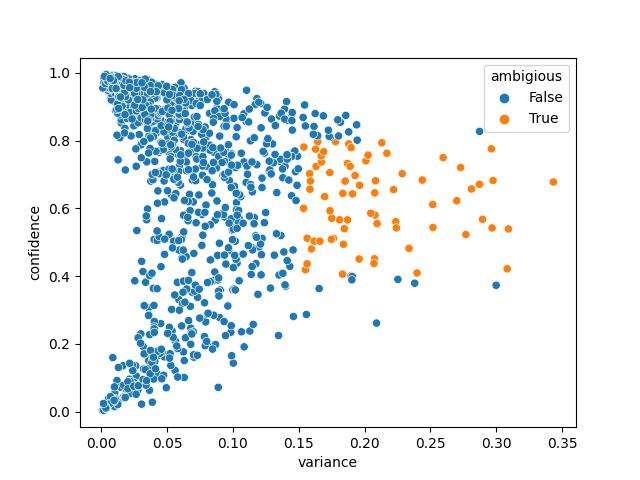
\includegraphics[width=\linewidth]{./ambiguous.jpg}
  \caption{Data Cartogram of 2000 training examples, orange ambiguous}
  \label{}
\end{figure}

\begin{figure}
  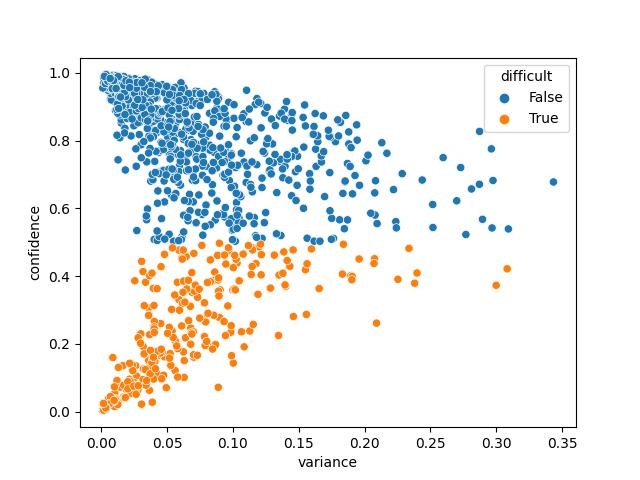
\includegraphics[width=\linewidth]{./difficult.jpg}
  \caption{Data Cartogram of 2000 training examples, orange difficult}
  \label{}
\end{figure}

\subsection{Dataset Cartography}

Training on labels that are ambiguous, that have high variablity, should in
theory help with this issue, even more so than hard to learn labels. An
ambiguous label is defined as a label that has high variance when predicted by
different iterations of the model. For example, a model that is trained on 500
iterations would predict the input differently than a model trained with 1000
iterations or a model trained with 1500 iterations. Furthermore, the average
confidence of that training example is not high or low.
\cite{swayamdipta2020dataset} We reproduced the code to analyze data, and have
plotted 500 training examples in figure 1. 

We believe that dataset cartography is a good fix to the problem. This is
because ambiguous training examples typically map to \enquote{hard} problems,
where as \enquote{hard to learn examples} typically map to training data with
errors. Therefore, we recommend training without \enquote{hard to learn}
examples and weighting \enquote{ambiguous} examples greater.

In order to deal with this, we first created a program that finds ambiguous
examples. We found the variance of the training example based on its confidence
of the gold label from a modeled trained on 500 iterations, 1000 iterations,
1500 iterations, 2000 iterations, 2500 iterations, and 3000 iterations. If the
variance was greater than 0.15, and the confidence of the model was in between
0.4 and 0.8, the example was deemed ambiguous. We further deemed labels with
confidence below 0.5 as \enquote{hard to learn} According to \textit{Swayamdipta
et al.}, training solely ambiguous examples leads to to greater performance than
training on the whole dataset, only easy to learn examples, or only hard to
learn examples. Thus it is logical to train on these examples. 

We pulled 1655 ambiguous samples from the training data and trained on those
examples. We trained for 15 epochs on ambiguous examples. As a test, we also
trained solely on difficult to learn examples for five epochs, of which there
were 6915, and benchmarked their performance.

\section{Evaluating Your Fix (25pt)}

\subsection{Ambiguous Examples}

We evaluated the new model that was trained on hard to learn examples and
independently trained on ambiguous examples. We found that models trained on
ambiguous examples tended to do better with more difficult data, but tended to
reduce the models overall average. For example, the accuracy of the model
trained on ambiguous data and tested on the contrast set was 80\%, whereas the
model that was not trained on ambiguous data had an accuracy of 77\%.

Based on manual evaluation of the contrast set, there is some evidence that the
model is able to reason better about differentiaing between entailment and
contradictions (given that they have no errors) and in some instances better
predicts neutrals. The following is a good example of this phenomenon:


\begin{quote}
premise: Under a blue sky with white clouds, a child reaches up to touch the propeller of a plane standing parked on a field of grass. \\
hypothesis: A child is not reaching to touch the propeller out of curiousity.  \\
label: neutral \\
predicted: neutral
\end{quote}

Unlike the the baseline model, which does not see the relationship that
\textit{not} has in the sentence (negating curiousity, not touching), the model
that is trained on ambiguous data is able to distinguish examples like these.

% Please add the following required packages to your document preamble:
% \usepackagemultirow
\begin{table}[]
    \caption{Ambiguous Trained Model on Contrast Set}
    \begin{tabular}{|ll|rrr|}
        \hline
        \multicolumn{2}{|l|}{\multirow{2}{*}{}}                           & \multicolumn{3}{l|}{\textbf{Predicted}}                                                              \\ \cline{3-5} 
        \multicolumn{2}{|l|}{}                                            & \multicolumn{1}{l|}{\textit{0}} & \multicolumn{1}{l|}{\textit{1}}  & \multicolumn{1}{l|}{\textit{2}} \\ \hline
        \multicolumn{1}{|l|}{\multirow{3}{*}{\textbf{True}}} & \textit{0} & \multicolumn{1}{r|}{90}         & \multicolumn{1}{r|}{7.692307692} & 0                               \\ \cline{2-5} 
        \multicolumn{1}{|l|}{}                               & \textit{1} & \multicolumn{1}{r|}{10}         & \multicolumn{1}{r|}{61.53846154} & 30.76923077                     \\ \cline{2-5} 
        \multicolumn{1}{|l|}{}                               & \textit{2} & \multicolumn{1}{r|}{0}          & \multicolumn{1}{r|}{7.692307692} & 92.30769231                     \\ \hline
    \end{tabular}
    \caption*{\textit{ 0=Entailment, 1=Neutral, 2=Contradiction }}
\end{table}

% Please add the following required packages to your document preamble:
% \usepackage{multirow}
\begin{table}[]
    \caption{Ambiguous Trained Model on Validation Set}
    \begin{tabular}{|ll|rrr|}
        \hline
        \multicolumn{2}{|l|}{\multirow{2}{*}{}}                           & \multicolumn{3}{l|}{\textbf{Predicted}}                                                             \\ \cline{3-5} 
        \multicolumn{2}{|l|}{}                                            & \multicolumn{1}{l|}{\textit{0}} & \multicolumn{1}{l|}{\textit{1}} & \multicolumn{1}{l|}{\textit{2}} \\ \hline
        \multicolumn{1}{|l|}{\multirow{3}{*}{\textbf{True}}} & \textit{0} & \multicolumn{1}{r|}{83.53}      & \multicolumn{1}{r|}{9.79}       & 7.04                            \\ \cline{2-5} 
        \multicolumn{1}{|l|}{}                               & \textit{1} & \multicolumn{1}{r|}{6.39}       & \multicolumn{1}{r|}{79.75}      & 13.48                           \\ \cline{2-5} 
        \multicolumn{1}{|l|}{}                               & \textit{2} & \multicolumn{1}{r|}{2.70}       & \multicolumn{1}{r|}{7.48}       & 89.871                          \\ \hline
    \end{tabular}
    \caption*{\textit{ 0=Entailment, 1=Neutral, 2=Contradiction }}
\end{table}

However, the model that was trained on ambiguous data seemed to suffer on the
overall benchmark of the evaluation set. The accuracy dropped from 88\% to 84\%
on the validation set. Table 5 and 6 show the accuracy of the ambiguously
trained model on the contrast and validation set, and shows that there is
improvement in contrast set but some regression in the validation set.

\subsection{Difficult to learn examples}

Unsurprisingly, difficult to learn examples had accuracies that were
significantly lower than the base model. However, it was surpring the extent to
which they degraded the performance of the model. Like the ambiguous examples,
the difficult to learn examples were trained directly on top of the base model,
so the model was already partially fine tuned. Nevertheless, the 6915 training
examples over 5 epochs degraded the model performance a very large amount. The
accuracy of that model was significantly lower than base model, clocking in an
accuracy of 13\%. Even a model with random guessing could have done better.
Because of this, we highly suggest removing difficult to learn examples from the
training data. 

Due to time constraints, more ambiguous labels could not be extracted, but it's
certainly possible that if all 500000 training examples are indexed and
ambiguous ones are found, that the model could have better performance than it
currently does. Furthremore, it is clear that training only on diffult to learn
examples degrades model performance significantly.

 \section{Related Work (5pt)}
Zhang et al. \cite{zhang2022cartography} propose another algorithm that uses
data cartography called \enquote{cartography active learning}. However, their
approach differs slightly in that they actively select ambiguous and difficult
examples \textit{during} training and then adjust the input of the training in
real time to train on the ambiguous data. In contrast, our approach finds
ambiguous and difficult data after an initial training period and then trains on
that data.

\section{Conclusion (5pt)}

In this paper, we evaluate an ELECTRA based ML model on the Stanford Natural
Language Inference dataset. We find that the model has difficulty
differentiating between neutral labels and other classes and that it finds at
times spurious correlations between the premise and hypothesis. We also find
that the model suffers significant performance degradation when tested against a
contrast set. To remedy this, we recommend finding ambiguous labels (labels with
high variablity and medium conference) using data cartography, and train the
model on those data points in addition to the training set. Although not a
perfect method, training on ambiguous labels can help the model learn more
difficult correlations. We also suggest removing \enquote{difficult to learn}
training examples, as they hurt model performance and are likely annotator
errors. Dataset cartography overall is a highly effective method eliminating
unwanted training examples or weight wanted training examples.

\bibliography{sample}{}
\bibliographystyle{plain}


\end{document}
